\protect\hyperlink{main-nav}{≡} \protect\hyperlink{close-nav}{×}

\hypertarget{chapter-2-the-derivative}{%
\section{Chapter 2: The Derivative}\label{chapter-2-the-derivative}}

\textbf{Note: The videos for sections 2.1-2.5 were recorded based on an
older edition of the book. This means that some of the section numbers I
mention will no longer correspond to the same material, and screen-shots
may look different. However, the content is essentially the same, and
I've tried to put the videos in the correct location based on where the
material was moved.}

\hypertarget{introduction}{%
\subsection{Introduction}\label{introduction}}

\hypertarget{precalculus-idea-slope-and-rate-of-change}{%
\subsubsection{Precalculus Idea: Slope and Rate of
Change}\label{precalculus-idea-slope-and-rate-of-change}}

The slope of a line measures how fast a line rises or falls as we move
from left to right along the line. It measures the rate of change of the
y-coordinate with respect to changes in the x-coordinate. If the line
represents the distance traveled over time, for example, then its slope
represents the velocity. In the figure, you can remind yourself of how
we calculate slope using two points on the line:

\begin{figure}
\centering
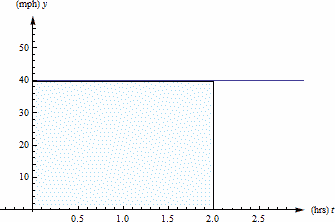
\includegraphics{images/image001.png}
\caption{\textbackslash{}( m=\textbackslash{}text\{Slope from
\textbackslash{}( P \textbackslash{}) to \textbackslash{}( Q
\textbackslash{})\}=\textbackslash{}dfrac\{\textbackslash{}text\{rise\}\}\{\textbackslash{}text\{run\}\}=\textbackslash{}dfrac\{y\_2-y\_1\}\{x\_2-x\_1\}=\textbackslash{}dfrac\{\textbackslash{}Delta
y\}\{\textbackslash{}Delta x\}\textbackslash{})}
\end{figure}

We would like to be able to get that same sort of information (how fast
the curve rises or falls, velocity from distance) even if the graph is
not a straight line. But what happens if we try to find the slope of a
curve, as in the figure below?

\begin{figure}
\centering
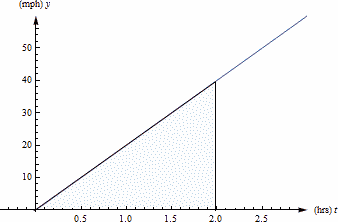
\includegraphics{images/image002.png}
\caption{}
\end{figure}

We need two points in order to determine the slope of a line. How can we
find a slope of a curve, at just one point? The answer, as suggested in
the figure, is to find the slope of the tangent line to the curve at
that point. Most of us have an intuitive idea of what a tangent line is.
Unfortunately, ``tangent line'' is hard to define precisely.

\hypertarget{definition-secant-line}{%
\paragraph{Definition (Secant Line)}\label{definition-secant-line}}

A \textbf{secant line} is a line between two points on a curve

See the image below:

\begin{figure}
\centering
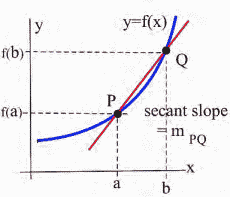
\includegraphics{images/image111.png}
\caption{}
\end{figure}

\hypertarget{cant-quite-do-it-yet-definition-tangent-line}{%
\paragraph{Can't-quite-do-it-yet Definition (Tangent
Line)}\label{cant-quite-do-it-yet-definition-tangent-line}}

A \textbf{tangent line} is a line at one point on a curve\ldots{} that
does its best to be the curve at that point?

As you may be able to see in the image below, the closer the point
\textbackslash{}(Q\textbackslash{}) is to the point
\textbackslash{}(P\textbackslash{}), the closer the secant slope gets to
the tangent slope. This will be key to finding the tangent slope, but
first we need to more carefully define the idea of ``getting closer
to.''

\begin{figure}
\centering
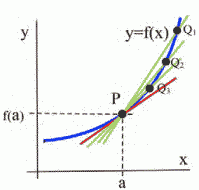
\includegraphics{images/image112.png}
\caption{}
\end{figure}

\hypertarget{section-2.1-limits-and-continuity}{%
\section{Section 2.1: Limits and
Continuity}\label{section-2.1-limits-and-continuity}}

\hypertarget{limits}{%
\subsection{Limits}\label{limits}}

In the last section, we saw that as the interval over which we
calculated got smaller, the secant slopes approached the tangent slope.
The \textbf{limit} gives us better language with which to discuss the
idea of ``approaches.''

The limit of a function describes the behavior of the function when the
variable is near, but does not equal, a specified number (see the figure
below).

\begin{figure}
\centering
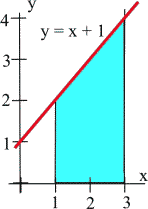
\includegraphics{images/image011.png}
\caption{}
\end{figure}

\hypertarget{definition-limit}{%
\paragraph{Definition (Limit)}\label{definition-limit}}

If the values of \textbackslash{}(f(x)\textbackslash{}) get closer and
closer, as close as we want, to one number
\textbackslash{}(L\textbackslash{}) as we take values of
\textbackslash{}(x\textbackslash{}) very close to (but not equal to) a
number \textbackslash{}(c\textbackslash{}), then we say "\textbf{the
limit of \textbackslash{}(f(x)\textbackslash{}) as
\textbackslash{}(x\textbackslash{}) approaches
\textbackslash{}(c\textbackslash{}) is
\textbackslash{}(L\textbackslash{})}" and we write
\textbackslash{}{[}\textbackslash{}lim\textbackslash{}limits\_\{x\textbackslash{}to
c\} f(x)=L.\textbackslash{}{]} The symbol "\textbackslash{}(
\textbackslash{}to \textbackslash{})" means "approaches" or, less
formally, "gets very close to".

(This definition of the limit isn't stated as formally as it could be,
but it is sufficient for our purposes in this course.)

Note:

\begin{itemize}
\tightlist
\item
  \textbackslash{}(f(c)\textbackslash{}) is a single number that
  describes the behavior (value) of
  \textbackslash{}(f(x)\textbackslash{}) \textbf{at} the point
  \textbackslash{}(x = c\textbackslash{}).
\item
  \textbackslash{}(\textbackslash{}lim\textbackslash{}limits\_\{x\textbackslash{}to
  c\} f(x)\textbackslash{}) is a single number that describes the
  behavior of \textbackslash{}(f(x)\textbackslash{}) near, \textbf{but
  NOT at}, the point \textbackslash{}(x = c\textbackslash{}).
\end{itemize}

If we have a graph of the function near x = c, then it is usually easy
to determine \textbackslash{}(
\textbackslash{}lim\textbackslash{}limits\_\{x\textbackslash{}to c\}
f(x) \textbackslash{}).

(Here is a link to the pictures used in the following video as well as
elsewhere in this chapter:
\href{otherfiles/graphs_for_limit_and_continuity_videos_math141.pdf}{Graphs
for Limits and Continuity Examples}.)

To view this video please enable JavaScript, and consider upgrading to a
web browser that \href{http://videojs.com/html5-video-support/}{supports
HTML5 video}

\hypertarget{example-1}{%
\paragraph{Example 1}\label{example-1}}

Use the graph of \textbackslash{}(y = f(x)\textbackslash{}) in the
figure below to determine the following limits:

\begin{enumerate}
\tightlist
\item
  \textbackslash{}(\textbackslash{}lim\textbackslash{}limits\_\{x\textbackslash{}to
  1\} f(x)\textbackslash{})
\item
  \textbackslash{}(\textbackslash{}lim\textbackslash{}limits\_\{x\textbackslash{}to
  2\} f(x)\textbackslash{})
\item
  \textbackslash{}(\textbackslash{}lim\textbackslash{}limits\_\{x\textbackslash{}to
  3\} f(x)\textbackslash{})
\item
  \textbackslash{}(\textbackslash{}lim\textbackslash{}limits\_\{x\textbackslash{}to
  4\} f(x)\textbackslash{})
\end{enumerate}

\begin{figure}
\centering
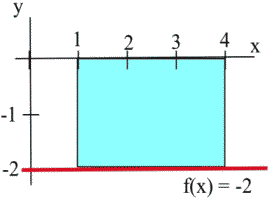
\includegraphics{images/image012.png}
\caption{}
\end{figure}

\begin{enumerate}
\tightlist
\item
  When \textbackslash{}(x\textbackslash{}) is very close to 1, the
  values of \textbackslash{}(f(x)\textbackslash{}) are very close to
  \textbackslash{}(y = 2\textbackslash{}). In this example, it happens
  that \textbackslash{}(f(1) = 2\textbackslash{}), but that is
  \textbf{irrelevant} for the limit. The only thing that matters is what
  happens for \textbackslash{}(x\textbackslash{}) \emph{close to} 1 but
  \textbackslash{}(x \textbackslash{}neq 1\textbackslash{}).
\item
  \textbackslash{}(f(2)\textbackslash{}) is undefined, but we only care
  about the behavior of \textbackslash{}(f(x)\textbackslash{}) for
  \textbackslash{}(x\textbackslash{}) \emph{close to} 2 but \emph{not
  equal to} 2. When \textbackslash{}(x\textbackslash{}) is close to 2,
  the values of \textbackslash{}(f(x)\textbackslash{}) are close to 3.
  If we restrict \textbackslash{}(x\textbackslash{}) close enough to 2,
  the values of \textbackslash{}(y\textbackslash{}) will be as close to
  3 as we want, so \textbackslash{}(
  \textbackslash{}lim\textbackslash{}limits\_\{x\textbackslash{}to 2\}
  f(x) = 3 \textbackslash{}).
\item
  When \textbackslash{}(x\textbackslash{}) is close to 3 (or "as
  \textbackslash{}(x\textbackslash{}) approaches the value 3"), the
  values of \textbackslash{}(f(x)\textbackslash{}) are close to 1 (or
  "approach the value 1"), so \textbackslash{}(
  \textbackslash{}lim\textbackslash{}limits\_\{x\textbackslash{}to 3\}
  f(x) = 1 \textbackslash{}). For this limit it is completely irrelevant
  that \textbackslash{}(f(3) = 2\textbackslash{}), We only care about
  what happens to \textbackslash{}(f(x)\textbackslash{}) for
  \textbackslash{}(x\textbackslash{}) close to and not equal to 3.
\item
  This one is harder and we need to be careful. When
  \textbackslash{}(x\textbackslash{}) is close to 4 and slightly less
  than 4 (\textbackslash{}(x\textbackslash{}) is just to the left of 4
  on the \textbackslash{}(x\textbackslash{})-axis), then the values of
  \textbackslash{}(f(x)\textbackslash{}) are close to 2. But if
  \textbackslash{}(x\textbackslash{}) is close to 4 and slightly larger
  than 4 then the values of \textbackslash{}(f(x)\textbackslash{}) are
  close to 3. If we only know that \textbackslash{}(x\textbackslash{})
  is very close to 4, then we cannot say whether \textbackslash{}(y =
  f(x)\textbackslash{}) will be close to 2 or close to 3--it depends on
  whether \textbackslash{}(x\textbackslash{}) is on the right or the
  left side of 4. In this situation, the
  \textbackslash{}(f(x)\textbackslash{}) values are not close to a
  single number so we say \textbackslash{}(f(x)\textbackslash{}) does
  not exist. It is irrelevant that \textbackslash{}(f(4) =
  1\textbackslash{}). The limit, as \textbackslash{}(x\textbackslash{})
  approaches 4, would still be undefined if
  \textbackslash{}(f(4)\textbackslash{}) was 3 or 2 or anything else.
\end{enumerate}

We can also explore limits using tables and using algebra.

To view this video please enable JavaScript, and consider upgrading to a
web browser that \href{http://videojs.com/html5-video-support/}{supports
HTML5 video}

\hypertarget{example-2}{%
\paragraph{Example 2}\label{example-2}}

Find \textbackslash{}(
\textbackslash{}lim\textbackslash{}limits\_\{x\textbackslash{}to 1\}
\textbackslash{}dfrac\{2x\^{}2-x-1\}\{x-1\} \textbackslash{}).

You might try to evaluate at \textbackslash{}(x = 1\textbackslash{}),
but \textbackslash{}(f(x)\textbackslash{}) is not defined at
\textbackslash{}(x = 1\textbackslash{}). It is tempting, \textbf{but
incorrect}, to conclude that this function does not have a limit as
\textbackslash{}(x\textbackslash{}) approaches 1.

{Using tables:} Trying some "test" values for x which get closer and
closer to 1 from both the left and the right, we get

\begin{longtable}[]{@{}ll@{}}
\toprule
\endhead
\textbackslash{}( x \textbackslash{}) & \textbackslash{}( f(x)
\textbackslash{})\tabularnewline
0.9 & 2.82\tabularnewline
0.9998 & 2.9996\tabularnewline
0.999994 & 2.999988\tabularnewline
0.9999999 & 2.9999998\tabularnewline
\textbackslash{}( \textbackslash{}to 1 \textbackslash{}) &
\textbackslash{}( \textbackslash{}to 3 \textbackslash{})\tabularnewline
\bottomrule
\end{longtable}

\begin{longtable}[]{@{}ll@{}}
\toprule
\endhead
\textbackslash{}( x \textbackslash{}) & \textbackslash{}( f(x)
\textbackslash{})\tabularnewline
1.1 & 3.2\tabularnewline
1.003 & 3.006\tabularnewline
1.0001 & 3.0002\tabularnewline
1.000007 & 3.000014\tabularnewline
\textbackslash{}( \textbackslash{}to 1 \textbackslash{}) &
\textbackslash{}( \textbackslash{}to 3 \textbackslash{})\tabularnewline
\bottomrule
\end{longtable}

The function \textbackslash{}(f\textbackslash{}) is not defined at
\textbackslash{}(x = 1\textbackslash{}), but when
\textbackslash{}(x\textbackslash{}) is close to 1, the values of
\textbackslash{}(f(x)\textbackslash{}) are getting very close to 3. We
can get \textbackslash{}(f(x)\textbackslash{}) as close to 3 as we want
by taking \textbackslash{}(x\textbackslash{}) very close to 1 so
\textbackslash{}{[}\textbackslash{}lim\textbackslash{}limits\_\{x\textbackslash{}to
1\} \textbackslash{}dfrac\{2x\^{}2-x-1\}\{x-1\}=3.\textbackslash{}{]}

{Using algebra:} We could have found the same result by noting that
\textbackslash{}{[} f(x)= \textbackslash{}dfrac\{2x\^{}2-x-1\}\{x-1\} =
\textbackslash{}dfrac\{(2x+1)(x-1)\}\{(x-1)\} = 2x+1\textbackslash{}{]}
as long as \textbackslash{}(x \textbackslash{}neq 1\textbackslash{}).
(If \textbackslash{}(x\textbackslash{}neq 1\textbackslash{}), then
\textbackslash{}(x--1 \textbackslash{}neq 0\textbackslash{}) so it is
valid to divide the numerator and denominator by the factor
\textbackslash{}(x--1\textbackslash{}).) The
"\textbackslash{}(x\textbackslash{}to 1\textbackslash{})" part of the
limit means that x is close to 1 but not equal to 1, so our division
step is valid and \textbackslash{}{[}
\textbackslash{}lim\textbackslash{}limits\_\{x\textbackslash{}to
1\}\textbackslash{}dfrac\{2x\^{}2-x-1\}\{x-1\} =
\textbackslash{}lim\textbackslash{}limits\_\{x\textbackslash{}to 1\}
2x+1 = 3,\textbackslash{}{]} which is our answer.

{Using a graph:} We can graph \textbackslash{}( y=f(x)=
\textbackslash{}dfrac\{2x\^{}2-x-1\}\{x-1\} \textbackslash{}) for
\textbackslash{}(x\textbackslash{}) close to 1:

\begin{figure}
\centering
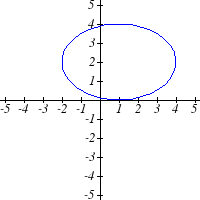
\includegraphics{images/image013.png}
\caption{}
\end{figure}

Notice that whenever \textbackslash{}(x\textbackslash{}) is close to 1,
the values of \textbackslash{}(y = f(x)\textbackslash{}) are close to 3.
Since \textbackslash{}(f\textbackslash{}) is not defined at
\textbackslash{}(x = 1\textbackslash{}), the graph has a hole above
\textbackslash{}(x = 1\textbackslash{}), but we only care about what
\textbackslash{}(f(x)\textbackslash{}) is doing for
\textbackslash{}(x\textbackslash{}) close to but \textbf{not equal to}
1.

To view this video please enable JavaScript, and consider upgrading to a
web browser that \href{http://videojs.com/html5-video-support/}{supports
HTML5 video}

\hypertarget{one-sided-limits}{%
\subsubsection{One Sided Limits}\label{one-sided-limits}}

Sometimes, what happens to us at a place depends on the direction we use
to approach that place. If we approach Niagara Falls from the upstream
side, then we will be 182 feet higher and have different worries than if
we approach from the downstream side. Similarly, the values of a
function near a point may depend on the direction we use to approach
that point.

\hypertarget{definition-left-and-right-limits}{%
\paragraph{Definition (Left and Right
Limits)}\label{definition-left-and-right-limits}}

The left limit of \textbackslash{}(f(x)\textbackslash{}) as
\textbackslash{}(x\textbackslash{}) approaches
\textbackslash{}(c\textbackslash{}) is
\textbackslash{}(L\textbackslash{}) if the values of
\textbackslash{}(f(x)\textbackslash{}) get as close to
\textbackslash{}(L\textbackslash{}) as we want when
\textbackslash{}(x\textbackslash{}) is very close to and \textbf{left of
\textbackslash{}(c\textbackslash{})} (i.e., \textbackslash{}(x
\textbackslash{}lt c\textbackslash{})). We write
\textbackslash{}{[}\textbackslash{}lim\textbackslash{}limits\_\{x\textbackslash{}to
c\^{}-\} f(x)=L.\textbackslash{}{]}

The right limit of \textbackslash{}(f(x)\textbackslash{}) as
\textbackslash{}(x\textbackslash{}) approaches
\textbackslash{}(c\textbackslash{}) is
\textbackslash{}(L\textbackslash{}) if the values of
\textbackslash{}(f(x)\textbackslash{}) get as close to
\textbackslash{}(L\textbackslash{}) as we want when
\textbackslash{}(x\textbackslash{}) is very close to and \textbf{right
of \textbackslash{}(c\textbackslash{})} (i.e., \textbackslash{}(x
\textbackslash{}gt c\textbackslash{})). We write
\textbackslash{}{[}\textbackslash{}lim\textbackslash{}limits\_\{x\textbackslash{}to
c\^{}+\} f(x)=L.\textbackslash{}{]}

\hypertarget{example-3}{%
\paragraph{Example 3}\label{example-3}}

Evaluate the one sided limits of the function
\textbackslash{}(f(x)\textbackslash{}) graphed below at
\textbackslash{}(x = 0\textbackslash{}) and \textbackslash{}(x =
1\textbackslash{}).

\begin{figure}
\centering
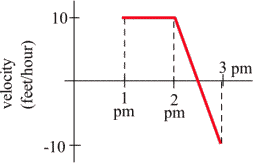
\includegraphics{images/image014.png}
\caption{}
\end{figure}

As \textbackslash{}(x\textbackslash{}) approach 0 from the \emph{left},
the value of the function is getting closer to 1, so \textbackslash{}(
\textbackslash{}lim\textbackslash{}limits\_\{x\textbackslash{}to
0\^{}-\} f(x) = 1. \textbackslash{})

As \textbackslash{}(x\textbackslash{}) approaches 0 from the
\emph{right}, the value of the function is getting closer to 2, so
\textbackslash{}(
\textbackslash{}lim\textbackslash{}limits\_\{x\textbackslash{}to
0\^{}+\} f(x) = 2. \textbackslash{})

Notice that since the limit from the left and limit from the right are
different, the general limit, \textbackslash{}(
\textbackslash{}lim\textbackslash{}limits\_\{x\textbackslash{}to 0\}
f(x) \textbackslash{}), does not exit.

At \textbackslash{}(x\textbackslash{}) approaches 1 from either
direction, the value of the function is approaching 1, so
\textbackslash{}{[}\textbackslash{}lim\textbackslash{}limits\_\{x\textbackslash{}to
1\^{}-\} f(x) =
\textbackslash{}lim\textbackslash{}limits\_\{x\textbackslash{}to
1\^{}+\} f(x) =
\textbackslash{}lim\textbackslash{}limits\_\{x\textbackslash{}to 1\}
f(x) = 1. \textbackslash{}{]}

To view this video please enable JavaScript, and consider upgrading to a
web browser that \href{http://videojs.com/html5-video-support/}{supports
HTML5 video}

\hypertarget{continuity}{%
\subsection{Continuity}\label{continuity}}

A function that is "friendly" and doesn't have any breaks or jumps in it
is called continuous. More formally,

\hypertarget{definition-continuity-at-a-point}{%
\paragraph{Definition (Continuity at a
Point)}\label{definition-continuity-at-a-point}}

A function \textbackslash{}(f(x)\textbackslash{}) is continuous at
\textbackslash{}(x = a \textbackslash{}) if and only if
\textbackslash{}(
\textbackslash{}lim\textbackslash{}limits\_\{x\textbackslash{}to a\}
f(x) = f(a)\textbackslash{}).

The graph below illustrates some of the different ways a function can
behave at and near a point, and the table contains some numerical
information about the function and its behavior.

\begin{figure}
\centering
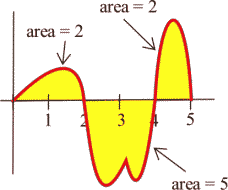
\includegraphics{images/image015.png}
\caption{}
\end{figure}

Based on the information in the table, we can conclude that
\textbackslash{}(f\textbackslash{}) is continuous at 1 since
\textbackslash{}(
\textbackslash{}lim\textbackslash{}limits\_\{x\textbackslash{}to 1\}
f(x) = 2 = f(1)\textbackslash{}). We can also conclude from the
information in the table that \textbackslash{}(f\textbackslash{}) is not
continuous at 2 or 3 or 4, because \textbackslash{}(
\textbackslash{}lim\textbackslash{}limits\_\{x\textbackslash{}to 2\}
f(x) \textbackslash{}neq f(2) \textbackslash{}), \textbackslash{}(
\textbackslash{}lim\textbackslash{}limits\_\{x\textbackslash{}to 3\}
f(x) \textbackslash{}neq f(3) \textbackslash{}), and \textbackslash{}(
\textbackslash{}lim\textbackslash{}limits\_\{x\textbackslash{}to 4\}
f(x) \textbackslash{}neq f(4) \textbackslash{}).

The behaviors at \textbackslash{}(x = 2\textbackslash{}) and
\textbackslash{}(x = 4\textbackslash{}) exhibit a \textbf{hole} in the
graph, sometimes called a \textbf{removable discontinuity}, since the
graph could be made continuous by changing the value of a single point.
The behavior at \textbackslash{}( x = 3 \textbackslash{}) is called a
\textbf{jump discontinuity}, since the graph jumps between two values.

So which functions are continuous? It turns out pretty much every
function you've studied is continuous where it is defined:
\textbf{polynomial, radical, rational, exponential, and logarithmic
functions are all continuous where they are defined}. Moreover,
\textbf{any combination of continuous functions is also continuous}.

This is helpful, because the definition of continuity says that for a
continuous function, \textbackslash{}(
\textbackslash{}lim\textbackslash{}limits\_\{x\textbackslash{}to a\}
f(x) = f(a) \textbackslash{}). That means for a continuous function, we
can find the limit by \textbf{direct substitution} (evaluating the
function) if the function is continuous at
\textbackslash{}(a\textbackslash{}).

To view this video please enable JavaScript, and consider upgrading to a
web browser that \href{http://videojs.com/html5-video-support/}{supports
HTML5 video}

\hypertarget{example-4}{%
\paragraph{Example 4}\label{example-4}}

Evaluate using continuity, if possible:

\begin{enumerate}
\tightlist
\item
  \textbackslash{}(
  \textbackslash{}lim\textbackslash{}limits\_\{x\textbackslash{}to 2\}
  x\^{}3-4x \textbackslash{})
\item
  \textbackslash{}(
  \textbackslash{}lim\textbackslash{}limits\_\{x\textbackslash{}to 2\}
  \textbackslash{}dfrac\{x-4\}\{x+3\} \textbackslash{})
\item
  \textbackslash{}(
  \textbackslash{}lim\textbackslash{}limits\_\{x\textbackslash{}to 2\}
  \textbackslash{}dfrac\{x-4\}\{x-2\} \textbackslash{})
\end{enumerate}

\begin{enumerate}
\tightlist
\item
  The given function is polynomial, and is defined for all values of x,
  so we can find the limit by direct substitution:\textbackslash{}{[}
  \textbackslash{}lim\textbackslash{}limits\_\{x\textbackslash{}to 2\}
  x\^{}3-4x = 2\^{}3-4(2) = 0. \textbackslash{}{]}
\item
  The given function is rational. It is not defined at x = -3, but we
  are taking the limit as x approaches 2, and the function is defined at
  that point, so we can use direct substitution:\textbackslash{}{[}
  \textbackslash{}lim\textbackslash{}limits\_\{x\textbackslash{}to 2\}
  \textbackslash{}dfrac\{x-4\}\{x+3\} =
  \textbackslash{}dfrac\{2-4\}\{2+3\}= -\textbackslash{}dfrac\{2\}\{5\}.
  \textbackslash{}{]}
\item
  This function is not defined at x = 2, and so is not continuous at x =
  2. We cannot use direct substitution.
\end{enumerate}

\begin{longtable}[]{@{}ll@{}}
\toprule
\endhead
\href{../chapter1/section1-8.php}{← Previous Section} &
\href{section2-2.php}{Next Section →}\tabularnewline
\bottomrule
\end{longtable}
